\section{Optical RFFE Communication}
\label{cha:optical_rffe_comm}
The WiSpry WS1040 digital capacitor is adjusted using the MIPI RFFE (RF Front End) protocol. In order to simplify sweep-measurements, which are a large part of this project, it is advantageous to be able to adjust the capacitance from outside the anechoic chamber. As having a long copper cable running from the antenna to outside the chamber may disturb the measurement significantly, a fiber optic cable will be used for communication between computer and antenna. As the fiber optic cable contains no metal, it should be less disturbing to the measurements.

The RFFE protocol requires three signals:
\begin{description}
    \item[SDATA] Bi-directional serial data signal carrying ones and zeros from the master (PC) to the slave (WS1040) and back. Both the master and the slave can drive this line.
    \item[SCLK] Serial clock. The master both clocks data to and from the slave.
    \item[VIO] Reference voltage of \SI{1.8}{V}. The SDATA and SCLK signals swing from \SI{0}{V} to VIO so VIO is the common reference -- not ground!
\end{description}
The WS1040 chip is rated for a supply voltage between \SI{2.7}{V} and \SI{5.0}{V}, so the VIO voltage is generated separately for communication.

The purpose of this communication link is solely to write to registers in the WS1040 so only one-way communication is necessary. To minimize the number of fibers, it is chosen to communicate via UART (Universal Asynchronous Receiver/Transmitter) over the fiber and generate the RFFE signals locally by a microcontroller at the antenna side. This requires only one fiber to be connected. In case a response were required, two fibers could be connected.

\begin{figure}[htbp]
    \centering
    \includegraphics[scale=0.85]{img/optical_rffe/schematic_pc}
    \caption{Schematic for optical RFFE communication -- PC-side.}
    \label{fig:rffe_schematic_pc}
\end{figure}

\begin{figure}[htbp]
    \centering
    \includegraphics[scale=0.85]{img/optical_rffe/schematic_ant}
    \caption{Schematic for optical RFFE communication -- antenna-side.}
    \label{fig:rffe_schematic_ant}
\end{figure}

The schematics are shown in Figure~\ref{fig:rffe_schematic_pc} and Figure~\ref{fig:rffe_schematic_ant}. The design files for the board can be downloaded at \url{http://github.com/16gr1051}. Both the transmitter and receiver is included on the PC-side board. On the PC side, the RX and TX lines are connected to a PC using an USB to UART adapter (PC2102) with external connections for an FTDI breakout board. On the antenna side, the RFFE\_SCLK, RFFE\_SDATA, and Vrffe lines are connected to the WS1040 chip.

In the following, each part of the design is described.

\subsection{USB to Serial Adapter}
In order to communicate from the PC using UART, a USB-to-serial adapter (PC2102) is used. The input is simply a USB connection to the PC and the output is a RX and a TX line for the optical circuit. For redundancy, the circuit is laid out with connections for an external FTDI breakout board.

\subsection{Transmitter}
The transmitter is made up from an open-collector comparator. The UART TX signal is connected to the inverting input of the comparator and a voltage divider, dividing the supply range in half, is connected to the non-inverting input. This means that when the input-signal is high (above $V_{cc}/2$), the comparator will pull down the cathode of the LED down to ground, lighting up the LED. When the input-signal is low (below $V_{cc}/2$), the output of the comparator will be floating, and no current will run through the LED -- no light.

\subsection{Receiver}
The light detector (IF-D91) functions as a light-dependent current source. When lit, around \SI{3}{\micro\ampere} is supplied and when dark, around \SI{10}{nA} is supplied. When this current is supplied to a \SI{100}{k\ohm} resistor, the voltage will alter between \SI{300}{mV} (light) and \SI{1}{mV} (dark). The voltage divider on the inverting input is dimensioned to set a threshold in between of these two values. By the pull-up resistor on the output, this means that the output will be high when light is supplied to the light detector and the output will be low when no light is supplied.

\subsection{Microcontroller and Protocol}
The microcontroller is an Atmel ATmega168. It receives one-byte commands from the PC through UART at \SI{9600}{baud}, \SI{8}{bit}, no parity, one stop bit (9600 8N1). The commands are ASCII characters as described in Table~\ref{tab:rffe_commands}. The source code for the microcontroller can be downloaded at \url{http://github.com/16gr1051}.

\begin{table}[htbp]
    \centering
    \begin{tabular}{|l|l|r|l|}
        \hline
        UART command & Action & Value & Note \\
        \hline
        A & Set active slave address & \texttt{0b0111} & \\
        B & Set active slave address & \texttt{0b0110} & \\
        \hline
        x & Set active register & 1 & Capacitor 1\\
        y & Set active register & 2 & Capacitor 2\\
        z & Set active register & 3 & Capacitor 3\\
        t & Set active register & 4 & Capacitor 4\\
        \hline
        0 & Set register value & \texttt{0x00} & \SI{0.30}{pF}\\
        1 & Set register value & \texttt{0x01} & \SIrange{0.39}{0.48}{pF}\\
        2 & Set register value & \texttt{0x02} & \SI{0.66}{pF}\\
        3 & Set register value & \texttt{0x03} & \SIrange{0.75}{0.83}{pF}\\
        4 & Set register value & \texttt{0x04} & \SI{1.01}{pF}\\
        5 & Set register value & \texttt{0x05} & \SIrange{1.10}{1.19}{pF}\\
        6 & Set register value & \texttt{0x06} & \SI{1.37}{pF}\\
        7 & Set register value & \texttt{0x07} & \SIrange{1.46}{1.55}{pF}\\
        8 & Set register value & \texttt{0x08} & \SI{1.73}{pF}\\
        9 & Set register value & \texttt{0x09} & \SIrange{1.81}{1.90}{pF}\\
        a & Set register value & \texttt{0x0a} & \SI{2.08}{pF}\\
        b & Set register value & \texttt{0x0b} & \SIrange{2.17}{2.26}{pF}\\
        c & Set register value & \texttt{0x0c} & \SI{2.44}{pF}\\
        d & Set register value & \texttt{0x0d} & \SIrange{2.53}{2.62}{pF}\\
        e & Set register value & \texttt{0x0e} & \SI{2.79}{pF}\\
        f & Set register value & \texttt{0x0f} & \SIrange{2.88}{2.97}{pF}\\
        \hline
    \end{tabular}
    \caption{UART commands and the resulting action on the microcontroller.}
    \label{tab:rffe_commands}
\end{table}

Two possible addresses are valid for the WS1040, making it possible to communicate with two separate chips on the same bus. The address depends on the high/low state of the USID pin on the WS1040. The WS1040 contains four capacitors which can be set individually. The capacitance range can be increased by connecting capacitors in parallel.

\begin{figure}[htbp]
    \centering
    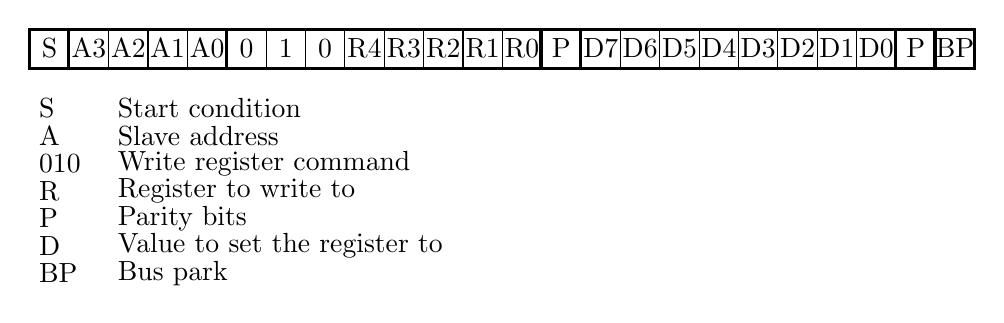
\begin{tikzpicture}[scale=0.5]
        \tikzstyle{bit} = [minimum height=5mm, minimum width=5mm, inner sep=0pt, draw];
        \foreach \i/\j in {
            0/S, 
            1/A3, 2/A2, 3/A1, 4/A0,
            5/0, 6/1, 7/0, 8/R4, 9/R3, 10/R2, 11/R1, 12/R0, 13/P,
            14/D7, 15/D6, 16/D5, 17/D4, 18/D3, 19/D2, 20/D1, 21/D0, 22/P,
            23/BP
        } {
            \node [bit,anchor=south west] at (\i,0) {\j};
        };

        \draw[very thick] (0,0) rectangle (1,1);
        \draw[very thick] (1,0) rectangle (5,1);
        \draw[very thick] (5,0) rectangle (13,1);
        \draw[very thick] (13,0) rectangle (14,1);
        \draw[very thick] (14,0) rectangle (22,1);
        \draw[very thick] (22,0) rectangle (23,1);
        \draw[very thick] (23,0) rectangle (24,1);

        \tikzstyle{T} = [anchor=west];
        \begin{scope}[yshift=-10mm, yscale=0.7]
            \foreach \i/\j/\l in {
                0/S/Start condition,
                1/A/Slave address,
                2/010/Write register command,
                3/R/Register to write to,
                4/P/Parity bits,
                5/D/Value to set the register to,
                6/BP/Bus park
            } {
                \node[T] at (0,-\i) {\j};
                \node[T] at (2,-\i) {\l};
            };
        \end{scope}
    \end{tikzpicture}
    \caption{RFFE command for writing to a register.}
    \label{fig:rffe_write_register}
\end{figure}
The RFFE command used for writing to a register is shown in Figure~\ref{fig:rffe_write_register}. The sequence is clocked out serially. A one bit is observed when the SCLK line goes high while the SDATA line is high and a zero bit is observed when the SCLK line goes high while the SDATA line is low. The start, parity, and bus park condition are described as follows:
\begin{description}
    \item[Start] SDATA pulses high while the SCLK line is kept low.
    \item[Parity] The parity is low if the number of ones in the preceding byte is odd. The parity is high if the number of ones in the preceding byte is even.
    \item[Bus park] SCLK is pulsed while SDATA is kept low (i.e.\ a zero is clocked out).
\end{description}
An example of and RFFE Write Register command is shown in Figure~\ref{fig:rffe_example}, where \texttt{0x00} is written to register 1 of the slave with address \texttt{0b0111}. This is the RFFE output when sending the string \texttt{"Ax0"} to the microcontroller, according to Table~\ref{tab:rffe_commands}.

\begin{figure}[htbp]
    \centering
    \includegraphics{img/optical_rffe/avr_rffe_reg1_0x00}
    \caption{Example of an RFFE command from the microcontroller.}
    \label{fig:rffe_example}
\end{figure}

\subsection{Level Shifting and WS1040 Interface}
The final part of the circuit is the interface towards the tuner. The microcontroller outputs signals between \SI{0}{V} and \SI{3.3}{V} which is not compatible with the tuner. Therefore, a level shifter is inserted, translating the \SI{3.3}{V} to \SI{1.8}{V}. The \SI{1.8}{V} is generated by a low-dropout voltage regulator.

\subsection{Testing}
An antenna board with tuner has been measured on a VNA and in the Satimo chamber, with and without the RFFE adaptor board to check if the $S$-parameters or total efficiency changes with the adaptor board present. The $S$-parameters and total efficiency, shown in Figure~\ref{fig:rffe_test_results}, shows no significant change when adding the RFFE adaptor board. The difference in the $S$-parameters may be because of slight bending due to handling of the antennas as the measurements were not done on the same day. The efficiency measurements were done the same day and shows no significant change. Another $S$-parameter measurement is shown in Figure~\ref{fig:rffe_test_results2} of another antenna. Here, the measurements are done in direct succession of each other and the $S$-parameters shows only \emph{very} little difference.

From the measurements just described, it has been verified that using the RFFE board with a fiber optic cable attached causes no significant change in $S$-parameters or total efficiency. Therefore, the board can be used for automating tests on a VNA and in the Satimo chamber.

\begin{figure}[htbp]
    \centering
    \begin{subfigure}[t]{0.49\linewidth}
        \includegraphics{img/optical_rffe/compare_sparams}
        \caption{$S$-parameters.} 
    \end{subfigure}
    \hfill
    \begin{subfigure}[t]{0.49\linewidth}
        \includegraphics{img/optical_rffe/compare_efficiency}
        \caption{Total efficiency.} 
    \end{subfigure}
    \caption{Comparison of the tuner PCB with and without the RFFE adaptor PCB.}
    \label{fig:rffe_test_results}
\end{figure}

\begin{figure}[htbp]
    \centering
    \includegraphics{img/optical_rffe/compare_sparams2}
    \caption{Comparison of $S$-parameters of the tuner PCB with and without RFFE adaptor PCB. }
    \label{fig:rffe_test_results2}
\end{figure}
